\documentclass{beamer}
\usepackage{verbatim}
\usetheme{Boadilla}
\title{CMBFAST}
\author{Floor Terra}
%\date{}

\begin{document}
	\begin{frame}
		\titlepage
	\end{frame} 
	
	\begin{frame}
		\frametitle{The big bang}
		\framesubtitle{A simple model}
		\begin{itemize}
			\item The universe starts small, hot and dense
			\item The universe expands and cools
			\item Recombination ($z=1100$, $T=4000K$)
			\item Surface of last scattering
			\item Universe expands while photons travel freely
			\item CMB is measured by Arno Penzias and Robert Woodrow Wilson 
			\begin{itemize}
				\item 1965 ($z=1$)
				\item Nobelprijs in 1978
			\end{itemize}
		\end{itemize}
	\end{frame}
	
	\begin{frame}
		\frametitle{WMAP}
		\framesubtitle{What do we see today?}
		\begin{center}
			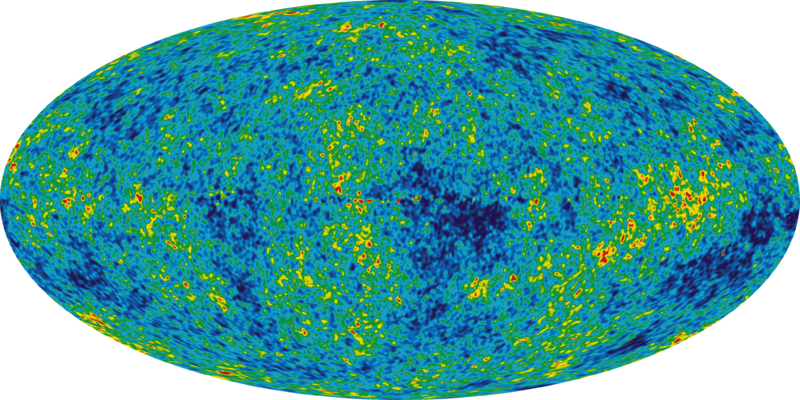
\includegraphics[width=90mm]{WMAP.png}

			\emph{WMAP 7 year  data}

			$T=2.725K$ fluctuations of order $10^{-5}$
		\end{center}
	\end{frame}
	
	\begin{frame}
		\frametitle{WMAP}
		\framesubtitle{The data}
		\begin{center}
			\includegraphics[width=90mm]{wmap_powerspectrum.png}

			\emph{http://map.gsfc.nasa.gov/media/080999/080999\_PowerSpectrumM.jpg}
		\end{center}
	\end{frame}
	
	\begin{frame}
		\frametitle{Perturbations}
		\framesubtitle{Where do they come from?}
		\begin{block}{Theory}
			\begin{itemize}
				\item Quantum fluctuations 
				\item Inflation
				\item Density fluctuations
			\end{itemize}
		\end{block}
		\begin{block}{CMBFAST}
			\begin{itemize}
				\item Plasma physics
				\item Gravitation and pressure
				\item Decoupling
				\item Last scattering surface
			\end{itemize}
		\end{block}
		\begin{block}{Today}
			\begin{itemize}
				\item Gravitation
				\item Large scale structure
			\end{itemize}
		\end{block}
	\end{frame}

	\begin{frame}[fragile]
		\frametitle{The calculations}
		\begin{columns}[c]
			\column{.4\textwidth}
			\tiny
			\begin{verbatim}
=============== CMBFAST Processing ===============
 
 CMB Parameters
 --------------
 ict      =     0
 lmo      =  2000   , akmax0   =  4000.00
 akmaxt   =     5.00, nlnkt    =     5
 ntf      =     1
 z(1)     =     0.00
 ndyn     =        0, wdyn     =    -1.00
 omegab   =     0.05, omegac   =     0.22
 omegav   =     0.73, omegan   =     0.00
 h0       =    70.00, tcmb     =     2.72
 yhe      =     0.24, annunr   =    3.04
 annunr   =     0.00, gsnunr   =     0.00
 rcflag   =        0
 riflag   =     1.00, optdlss  =     0.09
 zri      =    50.00, rif      =     0.20
 itflag   =     0   , nn       =     1
 itn      =     0   , irt      =     0
 an(1)         =     0.96
 alphans(1)    =     0.00
 ant(1)        =     0.00
 alphant(1)    =     0.00
 rat(1)        =     0.00
 lensflag =     0   , initfl   =     1

  Q_rms-ps =   0.5394E+02 micro K
			\end{verbatim}
			\column{.6\textwidth}
			\begin{center}
				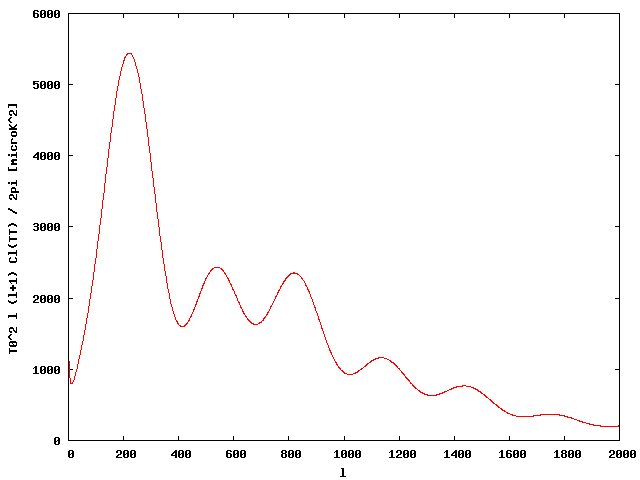
\includegraphics[width=70mm]{cmbfast_plot.png}
			
				\tiny http://lambda.gsfc.nasa.gov/toolbox/tb\_cmbfast\_form.cfm
			\end{center}
		\end{columns}
	\end{frame}

	\begin{frame}
		\frametitle{The CMBFAST code}
		\framesubtitle{A line-of-sight integration approach to cosmic microwave background anisotropies}
		\begin{itemize}
			\item Written by Uros Seljak and Matias Zaldarriaga.
			\item Article published in 1996
			\item The first fast CMB code
			\item Written in the FORTRAN programming language
		\end{itemize}
	\end{frame}
	
	\begin{frame}
		\frametitle{The problems with CMBFAST}
		\begin{columns}[c]
			\column{.6\textwidth}
			\begin{itemize}
				\item Sparse documentation
				\item Designed for interactive use
				\item FORTRAN
			\end{itemize}
			\column{.4\textwidth}
			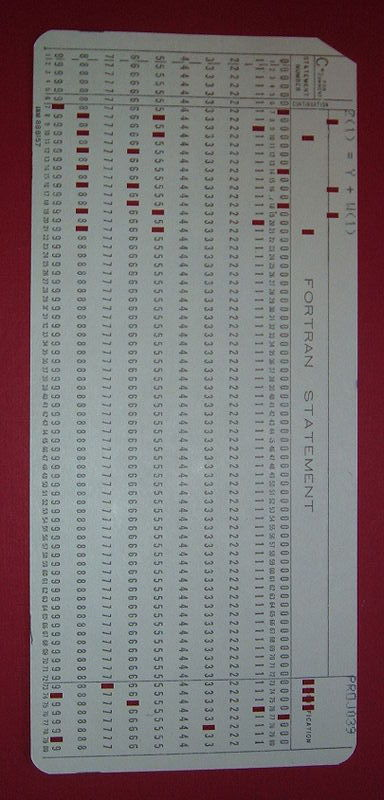
\includegraphics[width=30mm]{punch_card.jpg}
		\end{columns}
	\end{frame}
	
	\begin{frame}[fragile]
		\frametitle{py-cmbfast}
		\framesubtitle{A python wrapper around the CMBFAST code}
		\begin{itemize}
			\item Suited for both interactive and scripted use
			\item Easy to use
		\end{itemize}
		\begin{verbatim}
from libcmb import CMB
cmb = CMB()
# Generate a table with Bessel function values
cmb.jlgen(1500, 3000)
		\end{verbatim}
	\end{frame}

	\begin{frame}
		\frametitle{Goals}
		\begin{itemize}
			\item Finish wrapping all CMBFAST functionality
			\item Write a CMBFAST manual
			\item Write a small (improved) interactive interface
		\end{itemize}
	\end{frame}

	\begin{frame}
		\frametitle{Questions}
		\begin{center}
			
\includegraphics[width=90mm]{question.png}
		\end{center}
	\end{frame}


\end{document}
